\section{The parameters on the data}\label{sec:tuning}

The method has three kinds of parameters (Table~\ref{tab:parameters}). The \emph{tolerances} say
when two positions match: $\delta$, $\varepsilon_h$, $\varepsilon_z$, $\theta_{\max}$, $g$. The
\emph{duration} $\tau^*$ says how long a match must last to be a contact; it follows from the
share $q$ of chance contacts we accept (Section~\ref{sec:fdr}). The other \emph{settings} make the
computation exact or fast and are fixed by physical bounds. Each tolerance is compared with chance
through the null model of Section~\ref{sec:null}: the profiles of this section use a sample of
300 random dates, the choices of $\delta$ and $q$ the whole archive.

\begin{table}
\centering
\small
\begin{tabularx}{\textwidth}{@{}l l X@{}}
\toprule
Parameter & Value & How it was set \\
\midrule
$\delta$, largest delay & 2 min & measured on the delay profile, Section~\ref{sec:delta-choice} \\
$q$, accepted false discovery rate & 0.1 & trade-off, Section~\ref{sec:q} \\
$\tau^*$, shortest contact & 38.1 min & computed from $q$ and the null model, Section~\ref{sec:fdr} \\
$\varepsilon_h$, $\varepsilon_z$ & 500 m, 300 m & definitions: profiles without an edge, Section~\ref{sec:tolerances} \\
$g$, longest gap joined & 120 s & definition: gaps of real and chance contacts alike, Section~\ref{sec:tolerances} \\
$\theta_{\max}$ & 45$^\circ$ & no effect on the result, Section~\ref{sec:plateau} \\
$\Delta$, $h_{\max}$, $R_\dep$, $v_{\max}$, $R_s$, $r_{\min}$ & see Section~\ref{sec:fixed} & physical bounds and exactness \\
\bottomrule
\end{tabularx}
\caption{The parameters and how each was set.}
\label{tab:parameters}
\end{table}

\subsection{The maximum delay \texorpdfstring{$\delta$}{delta}}\label{sec:delta-choice}

Section~\ref{sec:delta} bounds $\delta$ by the visual range, at about 5~min. Here the data say
how long the delay between two pilots who fly together actually is.

\paragraph{The delay profile.} For every delay $l$, the correspondences $(t,t+l)$ of the real
pairs and of the surrogate pairs were counted, per second of exposure, with a window of 15~min on
300 random dates (58\,910~h of real exposure):
\begin{equation}\label{eq:profile}
  R(l)=\frac{\text{real correspondences at delay } l \text{ per second of exposure}}
             {\text{chance correspondences at delay } l \text{ per second of exposure}} .
\end{equation}
Chance is flat in the delay, as it should: a shifted copy has no preferred delay. The real
pairs peak at a few seconds, where they have 5.6 times the correspondences of chance, and
decay: $R$ falls below 4 at 105~s, below 3 at 195~s and below 2 at 500~s, and is still 1.5 at
15~min (Figure~\ref{fig:delays}). The excess has two parts. The fast one, within 2--3~min, is
pilots flying together. The slow one, which has not ended at 15~min, is pilots who use the
same thermals at about the same time without following each other, a synchrony that the
shifts of the surrogates remove. A rule such as ``the delay that holds 95\% of the excess''
would pick 13~min, because it counts the slow tail; that is why we read the ratio instead.

\begin{figure}
\centering
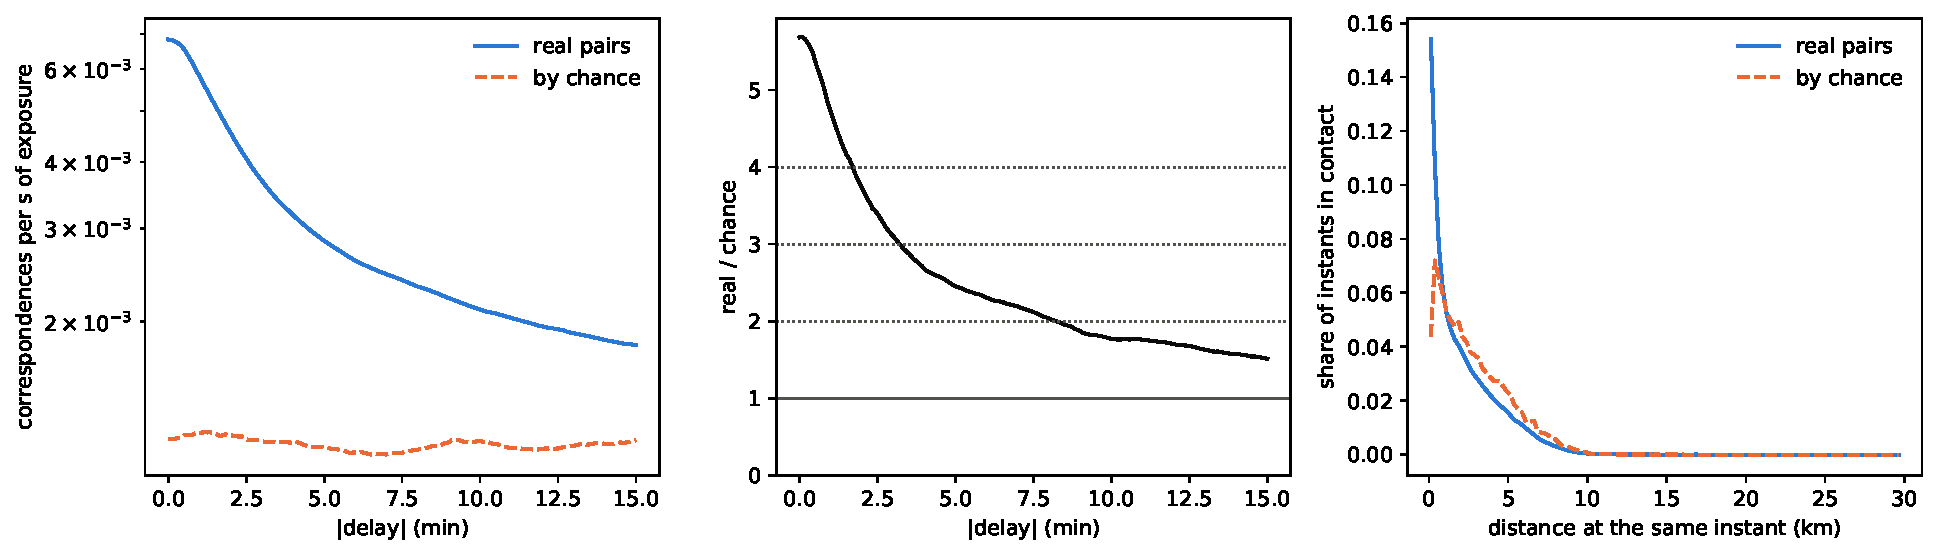
\includegraphics[width=\textwidth]{figures/assessment_delays.pdf}
\caption{The delay profile on 300 dates with a 15~min window. Left: correspondences per
second of exposure at each delay, real and by chance. Middle: their ratio $R(l)$ of
Eq.~\eqref{eq:profile}, with the levels 4, 3 and 2. Right: the distance between the two
pilots at the same instant when one is on the path of the other.}
\label{fig:delays}
\end{figure}

\paragraph{The delay inside the contacts.} The profile counts correspondences; this view looks at
the contacts themselves, through the delay $\ell_{\rm med}$ of each pair interval
(Section~\ref{sec:lag}). Its absolute value was computed for every pair interval of the run with
$\delta=5$~min, whose window is wide enough to show where the delays fall: 965\,770 intervals, of
which 169\,517 have all their instants in search and no delay.

\begin{table}
\centering
\small
\begin{tabular}{@{}l r c c c@{}}
\toprule
Duration of the interval & intervals & median $|\ell_{\rm med}|$ & within 2 min & at the edge \\
\midrule
under 10 min & 436\,575 & 210 s & 32\% & 29\% \\
10--30 min & 246\,587 & 160 s & 39\% & 12\% \\
30--90 min & 102\,357 & 80 s & 64\% & 2.1\% \\
90 min or more & 10\,734 & 25 s & 90\% & 6 intervals \\
\bottomrule
\end{tabular}
\caption{The delay of the pair intervals by their duration ($\delta=5$~min, whole archive). At
the edge: $|\ell_{\rm med}|\ge285$~s, the last 15~s of the window.}
\label{tab:ell}
\end{table}

\begin{figure}
\centering
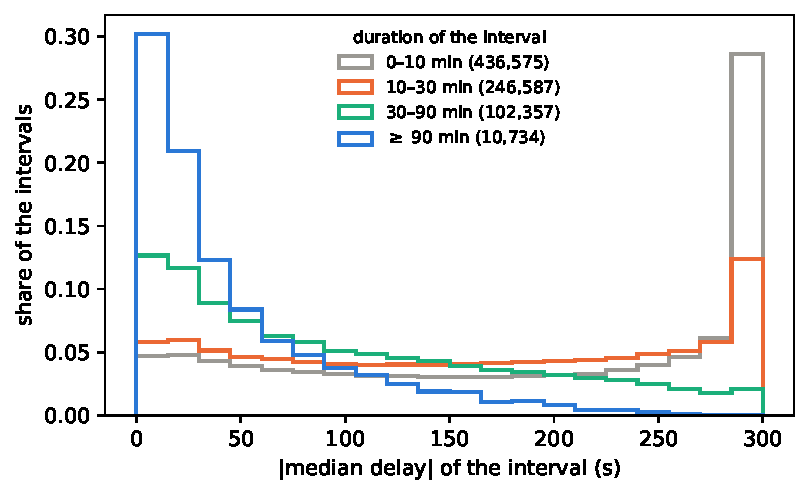
\includegraphics[width=0.62\textwidth]{figures/assessment_ell.pdf}
\caption{Distribution of the $|\ell_{\rm med}|$ of the pair intervals, by their duration
($\delta=5$~min, whole archive).}
\label{fig:ell}
\end{figure}

The longer the contact, the shorter the delay (Table~\ref{tab:ell}, Figure~\ref{fig:ell}). A
pair that only shares route and weather matches at any delay of the window, and its closest
correspondence is often at the largest ones: short intervals pile up at the edge, 29\% of
those under 10~min. The contacts of at least 90~min, all above $\tau^*$ of this run
(89.5~min), have a median delay of 25~s; 90\% of them lie within 2~min and only 6 of 10\,734
at the edge. Long contacts are pilots a few tens of seconds apart on the same path.

\paragraph{Choice.} We take $\delta=2$~min: within it the real correspondences are at least 3.7
times chance, and it contains nine in ten of the long contacts. Shortening the delay also
shortens $\tau^*$, since fewer chance matches enter: from 89.5 to 51.9~min at $q=0.05$
(Table~\ref{tab:q}).

\paragraph{Distance at the same instant.} The delay also bounds how far apart two pilots in
contact can be at the same instant: at most
$\varepsilon_h+v_{\max}\delta\approx0.5+27.8\times120/1000\approx3.8$~km. A separation of 6~km,
the largest we want to call a group, is never reached by one pair; a group, a chain of pairs, can
be wider. Even with the 15~min window, 58\% of the instants in contact have the two pilots within
2~km and 94\% within 6~km (Figure~\ref{fig:delays}, right).

The same distance was also counted without requiring a correspondence: at every grid instant when
both fly after departure, for all the real pairs and for the surrogates, on the dates of
Figure~\ref{fig:delays} that have surrogates (210 of 300, 58\,901~h of real exposure). Real pairs
are much closer than chance at short distance and have no edge (Figure~\ref{fig:separation}):
the ratio $g(d)$ is 10.4 within 100~m, below 2 from 500~m, below 1.5 from 900~m, below 1.1 from
2.7~km and below 1 from 5.7~km. Real pairs spend 6.6\% of their time together within 1~km of each
other, against 2.8\% by chance. Beyond 6~km $g$ falls slightly below 1, because both distributions
sum to one. The excess reaches several kilometres, beyond the visual range of 1.5~km of
Section~\ref{sec:delta}. Since the surrogates also change the hour, this excess may hold the
weather of the hour as well as sight, so it bounds neither the visual range nor the range of
following.

\begin{figure}
\centering
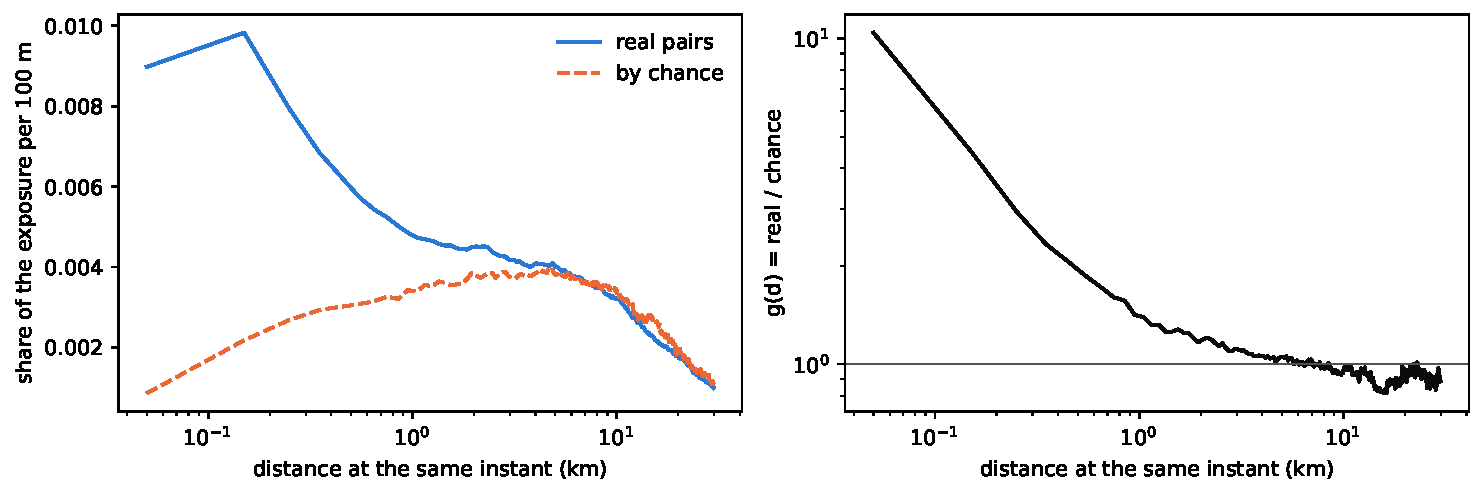
\includegraphics[width=\textwidth]{figures/assessment_separation.pdf}
\caption{Distance between the two pilots at the same instant, over all the time both fly, on
210 dates. Left: share of the exposure in each 100~m bin, real pairs and chance. Right: their
ratio $g(d)$.}
\label{fig:separation}
\end{figure}

\subsection{The tolerances against chance}\label{sec:tolerances}

In analogy with the delay profile, with $\delta=2$~min and the null model of the chosen run, at
every instant $t$ of pilot $i$ on the 210 dates of Figure~\ref{fig:separation}:
\begin{itemize}
\item the smallest horizontal distance between $i$ at $t$ and $j$ at $t+l$, $|l|\le\delta$,
  over the delays with $|z_i(t)-z_j(t+l)|<\varepsilon_z$ and headings that pass (left of
  Figure~\ref{fig:tolerances});
\item the smallest height difference over the delays with horizontal distance
  $<\varepsilon_h$ and headings that pass (middle);
\item the gaps between consecutive instants of contact of a pair (right).
\end{itemize}

\begin{figure}
\centering
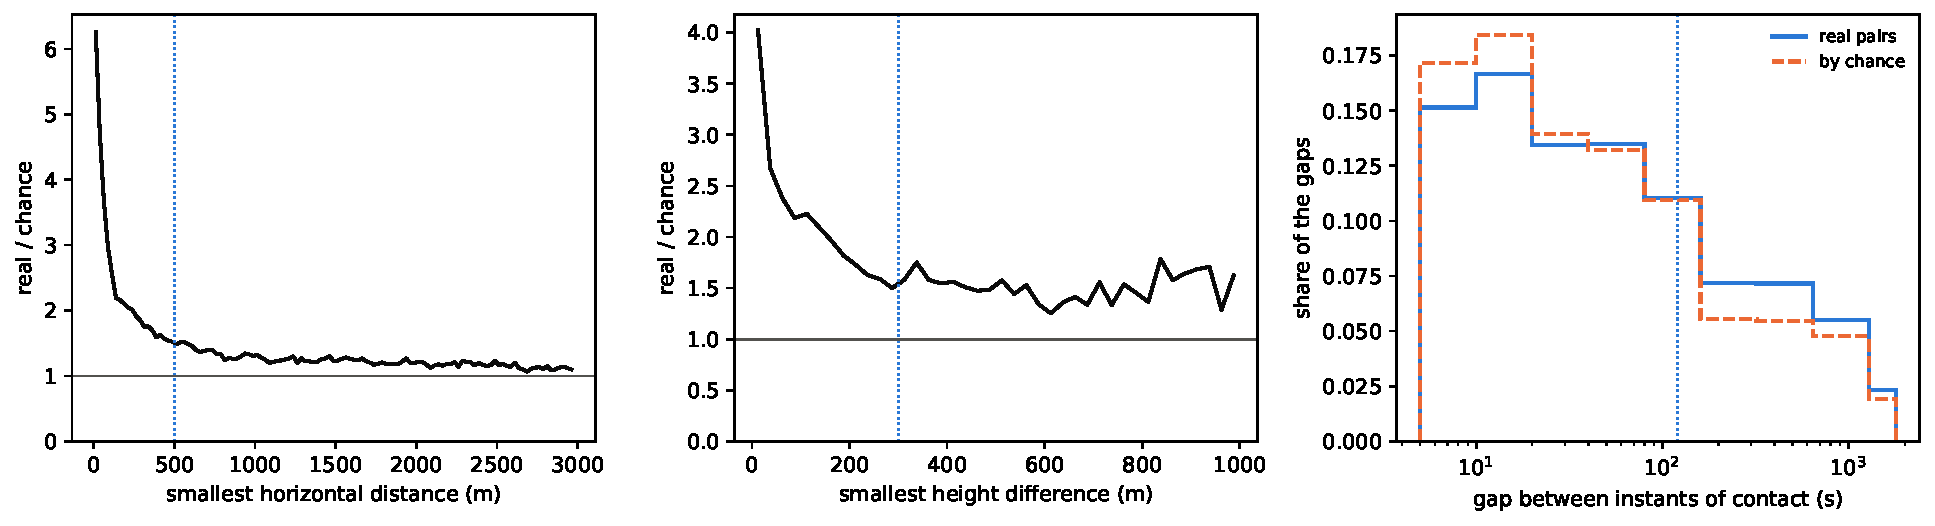
\includegraphics[width=\textwidth]{figures/assessment_tolerances.pdf}
\caption{The tolerance profiles on 210 dates. Left and middle: real pairs over chance, per
second of exposure, by the smallest horizontal distance and the smallest height difference to
the path of the other pilot within $\delta$; dotted, the values in use. Right: the lengths of
the gaps between instants of contact, as a share of all gaps (the 8\% of real and 9\% of chance
gaps longer than 30~min are not drawn); dotted, $g$.}
\label{fig:tolerances}
\end{figure}

None of the three has an edge (Figure~\ref{fig:tolerances}). The horizontal ratio is 6.3 within
25~m, below 2 from 250~m, below 1.5 from 500~m, and still 1.13 between 2.5 and 3~km. The
vertical ratio is 4.0 within 25~m and below 2 from 150~m; from 275~m on it stays near 1.5
(1.51 on average up to 1~km), the excess that the horizontal condition alone gives. Both values
in use sit where real pairs are about 1.5 times chance.

Real pairs have 1.46 times the gaps of chance per hour, because they have more contact, but the
lengths of the gaps are the same: the shares of each class differ by at most 2 points. The
gaps come from how pilots fly in and out of each other's path, the same in real and in chance
contacts, so the data do not single out $g$.

\subsection{One parameter at a time}\label{sec:plateau}

A plateau is a range of values of the tolerances around which the result does not change: a
value inside it makes the result insensitive to the exact threshold. If there is none, the
thresholds decide the result, and this must be said. The result is measured by $f_G$, the
fraction of the flight time after the departure spent in a group:
\begin{equation}\label{eq:fg}
  f_G=\frac{\sum_i\bigl|\{t\in T^\dep_i:\ \gamma_i(t)\notin\{\st{L},\st{S}\}\}\bigr|}{\sum_i|T^\dep_i|}.
\end{equation}
We changed one parameter at a time on 300 random dates, recalibrating $\tau^*$ each time, with
$\delta=5$~min (Table~\ref{tab:plateau}). $\theta_{\max}$ changes nothing: contacts in glide are
few. The others move $f_G$ by up to a factor three, mostly through $\tau^*$: there is no plateau,
in agreement with the profiles, and $\varepsilon_h$, $\varepsilon_z$ and $g$ are definitions. On
300 dates $\tau^*$ is noisy (126~min with the starting values against 89.5 on the whole archive,
and six settings stop at the same surrogate interval); a conclusive check needs the whole archive
for each setting, about one hour each. It was not repeated with $\delta=2$~min.

\begin{table}
\centering
\small
\begin{tabular}{@{}l c c c c@{}}
\toprule
Setting ($\delta=5$ min unless stated) & $\tau^*$ (min) & $f_G$ & episodes & flights in a group \\
\midrule
starting values & 126.1 & 0.034 & 98 & 210 \\
$\varepsilon_h=250$ m & 75.1 & 0.058 & 253 & 537 \\
$\varepsilon_h=1000$ m & 126.8 & 0.065 & 162 & 372 \\
$\varepsilon_z=150$ m & 126.1 & 0.020 & 61 & 125 \\
$\varepsilon_z=600$ m & 126.1 & 0.044 & 122 & 268 \\
$\delta=2$ min & 42.6 & 0.106 & 600 & 1\,170 \\
$\delta=10$ min & 128.4 & 0.062 & 153 & 365 \\
$\theta_{\max}=30^\circ$ & 126.1 & 0.034 & 97 & 208 \\
$\theta_{\max}=90^\circ$ & 126.1 & 0.034 & 98 & 210 \\
$g=60$ s & 75.8 & 0.087 & 332 & 732 \\
$g=300$ s & 126.1 & 0.055 & 141 & 318 \\
\bottomrule
\end{tabular}
\caption{One parameter at a time on 300 random dates (7\,051 flights), $q=0.05$.}
\label{tab:plateau}
\end{table}

\subsection{The false discovery rate \texorpdfstring{$q$}{q}}\label{sec:q}

$q$ is the share of chance contacts we accept among those we keep. A smaller $q$ keeps only
very long contacts and few groups, all of them real; a larger $q$ sees more groups, with more
chance among them. Table~\ref{tab:q} and Figure~\ref{fig:q} give the trade-off.

\begin{table}
\centering
\small
\begin{tabular}{@{}l l c c c c c@{}}
\toprule
$\delta$ & $q$ & $\tau^*$ (min) & 5--95\% over dates & para in a group & hang in a group & episodes \\
\midrule
5 min & 0.05 & 89.5 & 79.5--91.5 & 8.9\% & 2.1\% & 6\,090 \\
2 min & 0.05 & 51.9 & 49.1--53.3 & 13.7\% & 3.8\% & 10\,553 \\
2 min & 0.1  & 38.1 & 37.0--41.1 & 21.7\% & 6.9\% & 17\,169 \\
2 min & 0.2  & 26.4 & 25.2--27.2 & 31.7\% & 13.9\% & 26\,504 \\
\bottomrule
\end{tabular}
\caption{$\tau^*$ and the groups it gives. Flights with a logger of at most 10~s and a
position after departure: 154\,598 paragliders and 6\,039 hang gliders.}
\label{tab:q}
\end{table}

\begin{figure}
\centering
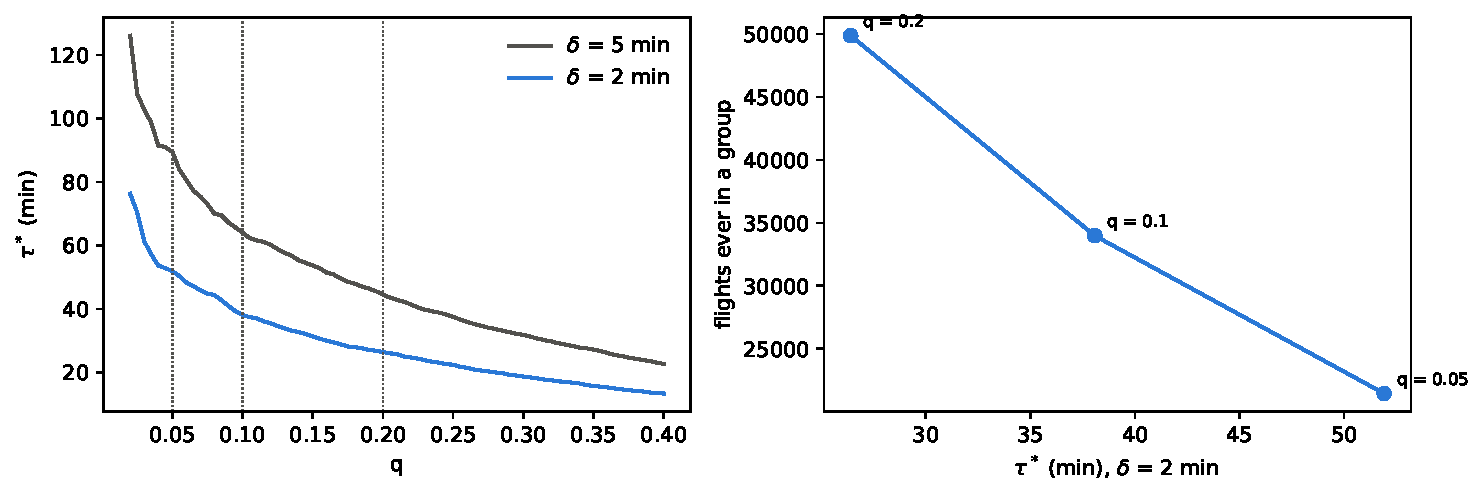
\includegraphics[width=\textwidth]{figures/assessment_q.pdf}
\caption{Left: $\tau^*$ as a function of $q$, for the two delays. Right: flights ever in a
group against $\tau^*$, for $q=0.05$, 0.1 and 0.2 with $\delta=2$~min.}
\label{fig:q}
\end{figure}

We take $q=0.1$: at most one contact in ten is chance, and $\tau^*=38.1$~min. Going to 0.2 would
lower $\tau^*$ to 26~min but would let chance make one group in five.

\subsection{Fixed settings}\label{sec:fixed}

\begin{itemize}
\item $\Delta=5$~s, the common grid: a pilot is at most 69~m from a grid position at
  100~km/h, against $\varepsilon_h=500$~m (Section~\ref{sec:phase0}).
\item $h_{\max}=10$~s: positions are interpolated only between fixes at most 10~s apart; the
  flights of coarser loggers are left out of the statistics.
\item $R_\dep=3$~km: contacts around the takeoff, before the first exit from this disc, are not
  counted (Section~\ref{sec:local}).
\item $v_{\max}=100$~km/h, the speed of the candidate filter: pieces of track end at every
  faster step, so the filter never misses a correspondence (Lemma~\ref{lem:filter}, checked
  against every pair of instants on synthetic days). The profiles of
  Section~\ref{sec:tolerances} widen the filter to 3~km, the largest distance they count.
\item $R_s=10$~km, $r_{\min}=2\delta+\Delta$, at most 200 surrogate pairs per date: the null
  model of Section~\ref{sec:null}.
\end{itemize}
